\documentclass[12pt,a4paper,oneside,openany,parskip=full,parindent=full]{book}
\usepackage[T1]{fontenc}
\usepackage[utf8]{inputenc}
\usepackage[polish]{babel}
\usepackage{graphicx}
\usepackage{times}
\usepackage{indentfirst}
\usepackage[left=3cm,right=2cm,top=2.5cm,bottom=2.5cm]{geometry}
\usepackage{natbib}
\usepackage{color}
\usepackage{xcolor}
\usepackage{tikz}
\usepackage{url}
\usepackage{dirtree}
\edef\restoreparindent{\parindent=\the\parindent\relax}
\usepackage{parskip}
\restoreparindent
\usepackage{listings}
\usepackage{enumerate}
\usepackage[hidelinks]{hyperref}

\definecolor{dkgreen}{rgb}{0,0.6,0}
\definecolor{gray}{rgb}{0.5,0.5,0.5}
\definecolor{mauve}{rgb}{0.58,0,0.82}

\lstset{frame=tb,
  language=Python,
  aboveskip=3mm,
  belowskip=3mm,
  showstringspaces=false,
  columns=flexible,
  basicstyle={\small\ttfamily},
  numbers=none,
  numberstyle=\tiny\color{gray},
  keywordstyle=\color{blue},
  commentstyle=\color{dkgreen},
  stringstyle=\color{mauve},
  breaklines=true,
  breakatwhitespace=true,
  tabsize=3
}


\frenchspacing
\linespread{1.5}
\addto\captionspolish{%
\renewcommand*\listtablename{Spis tabel}
\renewcommand*\tablename{Tabela}
}

\frenchspacing

\begin{document}

\begin{center}

\vspace{1cm}

Studium magisterskie
\end{center}

\vspace{1cm}

\noindent Kierunek: Informatyka

\vspace{1cm}

{
\leftskip=10cm\noindent
Michał Polakowski\newline
Nr albumu: 203446\newline
}

\vspace{2cm}

\title{Analiza porównawcza zastosowania współbieżności we frameworkach webowych FastAPI i Django}
\makeatletter

\begin{center}
\LARGE\bf
\@title
\end{center}

\vspace{2cm}

{
\leftskip=8cm\noindent
Praca magisterska\newline 
napisana w~Instytucie Matematyki, Fizyki i Informatyki\newline
pod kierunkiem naukowym\newline
Profa Dra rer. nat. Christopha Schwarzwellera
}

\vfill

\begin{center}
Gdańsk, \the\year
\end{center}
\thispagestyle{empty}

\clearpage
\thispagestyle{empty}
\clearpage

\tableofcontents

\clearpage
\chapter*{Streszczenie}
Moja praca opisuje dwie implementacje prostych mikroserwisów webowych, zaimplementowanych w dwóch różnych frameworkach. Oba mikroserwisy na żądanie wykonują operacje korzystające z mechanizmów zrównoleglania do wykonywania konkretnych operacji. Jednym z frameworków jest technologia FastAPI, drugim technologia Django.
\chapter{Wprowadzenie}

Wybór tematu mojej pracy jest ściśle związany z aktualnie panującymi trendami we współczesnym świecie programowania. Technologie asynchroniczne są w języku Python obecne w coraz większym stopniu i cieszą się rosnącą popularnością wśród programistów tego języka. Powodów takiego stanu rzeczy jest co najmniej kilka. 

Bogactwo frameworków webowych z wbudowaną obsługą asynchroniczności, coraz więcej współbieżnych modułów tworzonych przez społeczność do obsługi dotychczasowych sekwencyjnych funkcjonalności Pythona i wreszcie - coraz obszerniejsze wsparcie tego typu podejścia we wbudowanych bibliotekach języka oraz  w nim samym. Wymienione czynniki sprawiają, że uważam zajęcie się tą tematyką za pożyteczne.

Na początku pracy chciałbym zająć się szerzej tematem równoległości oraz współbieżności, gdyż pomimo że ogólnie pojęcia te bywają używane wymiennie, w mojej pracy będę je rozróżniał. Stąd też w pierwszych rozdziałach przedstawiam pokrótce ogólne definicje tych dwóch terminów i staram się rzetelnie nakreślić ich różnice.

W dalszej części pracy przedstawiam język Python. W mojej pracy skupiam się na jego konkretnej implementacji, którą jest CPython Znajomość krótkiej historii tej technologii będzie niezbędna, by zrozumieć pewnie mechanizmy, które na dość długo, a nawet po dziś dzień utrudniają pracę z Pythonem jako językiem współbieżnym. Dopiero jego najnowsze wersje wprowadziły do samej składni języka elementy ułatwiające zrozumienie działania mechanizmów asynchronicznych.

Kolejny rozdział poświęcam właśnie wspomnianym na końcu ostatniego akapitu mechanizmom. Jest ich co najmniej kilka i każdy ma swoją specyfikę pracy, wady oraz zalety. Mechanizmy te to mianowicie wbudowane moduły threading, multiprocessing oraz asyncio i powiązane z tym ostatnim słowa kluczowe async i await.

W rozdziale przedostatnim chciałbym zaprezentować sposoby użycia mechanizmów asynchronicznych w kontekście aplikacji webowej. Pierwszym wyborem ze względu na popularność tego frameworka względem jego dość krótkiego czasu istnienia jest FastAPI - uważany za jeden z najszybszych pythonowych frameworków webowych, do tego natywnie obsługujący asynchroniczność. Dla porównania zaprezentuję jak podobne zastosowanie byłoby rozwiązane w bardziej tradycyjnym frameworku, którym to w ninejszej pracy będzie Django.

Na koniec przeprowadzone eksperymenty opiszę i przedstawię w postaci wyników czasowych cyklu zapytanie-odpowiedź.

\textbf{Słowa kluczowe:} współbieżność, równoległość, aplikacje internetowe
\chapter{Współbieżność i równoległość}

Przewrotnie piewrszy rozdział mojej pracy o współbieżności zaczniemy od próby krótkiej definicji klasycznego sekwencyjnego programu komputerowego. Mianowicie program taki składa się z deklaracji danych i z zapisanych w jakmiś języku programowania instrukcji, które da się wykonać.\footnote{Mordechai Ben-Ari (1996). Podstawy programowania współbieżnego i rozproszonego, s.16} Instrukcje te są wykonywane przez komputer sekwencyjnie - jedna po drugiej, aż program dotrze do swojego końca.

W kontrze do programu sekwencyjnego stoją programy współbieżne. Są to programy, które abstrakcyjnie będą wykonywać wiele wspomnianych programów sekwencyjnych w tym samym czasie. Kwestię wspomnianej abstrakcyjności wyjaśnię dokładnie za chwilę, gdy poczynimy rozróżnienie na programy współbieżne oraz zrównoleglone\footnote{ang. odpowiednio concurrent oraz parallel}.

W dużym uproszczeniu możemy wyobrazić sobie dwa scenariusze, w których użycie współbieżności lub równoległości potencjalnie mogłoby przynieść nam jakies korzyści.

Pierwszym ze scenariuszy niech będzie kolejka w sklepie motoryzacyjnym. Stojąc w niej czekamy na obsłużenie nas przez asystenta sprzedaży. Następnie gdy nadchodzi nasza kolej składamy zamówienie, asystent przekierowuje nas do kasy abyśmy mogli zapłacić, a w tym samym czasie obsługa sklepu szuka dla nas zamówionego produktu. Po uiszczeniu opłaty oczekujemy na nasz produkt i pod jego znalezeniu i odbiorze możemy opuścić sklep.

Drugim scenariuszem jest sytuacja, gdy zbieramy się rano do pracy. Rozpoczynamy od wzięcia prysznica, następnie sporządzenia i zjedzenia śniadania, przygotowania ubrań i założenia ich, na końcu umycia zębów i wyjścia z mieszkania. Jest to lista czynności pomiędzy którymi nie zauważymy żadnych czasów oczekiwania (może z jakimś małym wyjątkiem oczekiwania na zagotowanie wody na kawę).

\section{Współbieżność}
Współbieżność jest terminem szerszym i zawierającym w sobie równoległość. 

W pierwszym scenariuszu jesteśmy programem, który ma dość dużo momentów ,,oczekiwania'' - stojąc w kolejce, czekając na produkt. W tym czasie oczekiwania możemy wykonywać jakąś inną czynność, na przykład pisać na wziętym z domu laptopie program, który musimy ukończyć do pracy. Po oczekiwaniu mamy swój opłacony paragon, który pokazujemy przy odbiorze produktu, więc nie martwiąc się o to że ktoś inny ,,ukradnie'' nasze zamówienie kończymy dotychczas wykonywaną pracę i dopiero wtedy odbieramy.

W scenariuszu drugim brak czasów oczekiwania sprawia, że w pojedynkę nie jesteśmy w stanie wykonać więcej czynności niż mamy zaplanowane. Przygotowując śniadanie nie możemy równocześnie w tym samym czasie przygotowywać ubrań, w które się następnie ubierzemy, a kiedy się w nie ubieramy brać jednocześnie prysznic.

Tak w uproszczeniu działają programy współbieżne. Jest to oczywiście pewna abstrakcja, która pozwala nam wyobrazić sobie swego rodzaju przełożenie idei współbieżności naświat rzeczywisty, gdyż faktyczna prędkość działań urządzeń elektronicznych jest bardzo trudna do ogarnięcia intuicyjnie.\footnote{Mordechai Ben-Ari (1996). Podstawy programowania współbieżnego i rozproszonego, s.17}

\section{Równoległość}
Równoległość jest podzbiorem współbieżności, którego charakterystyczną cechą jest brak pozorności współbieżności. Wszystkie procesy zaplanowane do wykonania w ramach programu, które mają się wykonać współbieżnie będą \emph{faktycznie} wykonywały się dokładnie w tym samym czasie. Warunkiem zaistnienia takiego stanu rzeczy jest posiadanie do dyspozycji więcej niż jednego procesora lub kilku jego rdzeni.

W przypadku naszego pierwszego scenariusza będzie to oznaczało, że asystentów sprzedaży jest kilku, więc kolejka i czas oczekiwania w niej jest skrócony. Asystenci odbierają nasze zamównienie. Asystent sprzedaży jest jednocześnie kasjerem, więc inkasuje od nas opłatę za zamówiony produkt, a następnie idzie go szukać. W tym czasie nasza uwaga skupiona jest w pełnie na staniu przy kasie i czoekiwaniu na produkt, nie jesteśmy w stanie wykorzystać tego czasu na wykonanie innej pracy.po znalezieniu produktu możemy opuścić sklep.

W scenariuszu drugim sytuacja będzie wyglądała inaczej. Jesteśmy my oraz naszych trzech pomocników, którzy zajmują się naszym domem. W czasie gdy my bierzemy prysznic, jeden z pomocników przygotowuje śniadanie, drugi prasuje koszulę i spodnie, a trzeci pastuje nasze buty. Zjadając śniadanie, widzimy, że jeden z pomocników w tym czasie zabrał się już za ogólne porządki, drugi wynosi śmieci, a trzeci przygotowuje produkty na obiad, który będzie gotowy, gdy wrócimy z pracy. Tacy pomocnicy to właśnie dodatkowe procesory naszej maszyny (lub rdzenie).
\chapter{Python}

\section{Krótka historia}
Pomimo tego, że Python uważany jest za jeden z nowocześniejszych współczesnych języków programowania to jego historia sięga aż końcówki lat '80 XX wieku. Jego pierwsza konkretna implementacja została rozpoczęta w grudniu 1989 roku przez Guido van Rossuma w Narodowym Instytucie Badań Matematyki i Informatyki w Holandii. Python miał być następcą języka ABC nad którym Guido van Rossum pracował od 1983 roku zanim zajął się Pythonem.\footnote{ "The Making of Python". Artima Developer. \url{https://www.artima.com/articles/the-making-of-python}, dostęp 18.06.2021}

Python po ABC odziedziczył ideę stania się językiem, który będzie skierowany do odbiorców niekoniecznie będących programistami lub osobami odpowiedzialnymi w jakikolwiek sposób za tworzenie oprogramowania. Dziś wydaje się, że ta idea została osiągnieta, gdyż Python jest jednym z najczęściej używanych języków w nauce poza informatyką. Przykładowo na szacunkowe 8.2 miliona użytkowników Pythona, z których aż 69\% to twórcy ML oraz badacze danych\footnote{ang. data scientists}.\footnote{\url{https://slashdata-website-cms.s3.amazonaws.com/sample_reports/ZAamt00SbUZKwB9j.pdf}, dostęp 16.06.2021}

Wersja Pythona z numerem 1.0 ujrzała światło dzienne w styczniu 1994 roku, ale wersja 0.9 istniała już od stycznia roku 1991 i posiadała system klas z dziedziczeniem, obsługę błędów, funkcje, oraz podstawowe typy danych takie jak ,,list'', ,,dict'' czy ,,str'', a także system modułów. W wersji 1.0 dodane zostały znane z języka Lisp funkcyjne narzędzie lambda, map, filter i reduce.

Wersja 2.0 wprowadziła jeden z charakterystycznych mechanizmów Pythona jakim jest list comprehension. Nie jest to całkowicie indywidualny twór twórców Pythona, gdyż podobne mechanizmy funkcjonowały - nomen omen - w funkcyjnych językach programowania takich jak SETL czy Haskell. to właśnie w trakcie tworzenia Pythona z dwójką z przodu zostały dodane takie elementy jak ,,nested scope'' czy ,,context manager'', pośród wielu innych zmian.

W roku 2014, gdy istniała już wersja 3 języka, zostało już oficjalnie ogłoszone, że Python 2.7 (czyli ostatnia wersja Python z dwójką z przodu) będzie wspierana do roku 2020 i zachęcano użytkowników języka do jak najszybszego przechodzenia na wersję 3. Ostatnie wydanie wersji 2 - dokładnie wersja 2.7.18 - została opublikowana 20 kwietnia 2020 roku i jest uważana za oficjalną datę zakończenia cyklu życia Pythona 2.

W międzyczasie od 3 grudnia 2008 roku równolegle z wersją 2 istniała i była rozwijana wersja 3 Pytona.\footnote{\url{https://www.python.org/download/releases/3.0/}} Jest to wersja aktualnie używana i wspierana, która co warto podkreślić, zepsuła kompatybiilność wsteczną względem wersji 2 i sprawiła, że przejścia z poprzedniej wersji na nową potrafiły byc w wypadku starszych aplikacji mocno czasochłonne. 

\section{Krótki opis}
Python jest językiem interpretowanym wysokopoziomowym ogólnego użytku. Przede wszystkim język ten kładzie nacisk na łatwość odczytu zapisanego w nim kodu. Łatwość tę osiągać ma poprzez użycie wcięć jako znaczących składniowo elementów języka.  Język ten jest dynamicznie typowany oraz korzysta z wbudwoanego ,,garbage collectora''. Wspiera co najmniej kilka paradygmatów programowania, w związku z czym pisząc w nim możemy używać paradygmatu proceduralnego, obiektowego lub funkcyjnego.

Bardzo rozbudowana biblioteka standardowa języka umożliwia bardzo szeroki zakres pracy z językiem, a dodatkowo społeczność cały czas tworzy i nadzoruje tworzenie modułów gotowych do pobrania za pomocą narzędzia pip. Dostępne do pobrania stworzone przez społeczność technologie możemy znaleźć na stronie https://pypi.org/.\footnote{\url{https://pypi.org/}} Jak już wspominałem wcześniej popularność w dziedzinach związanych z analizą danych, uczeniem maszynowym czy sztuczną inteligencją Python zawdzięcza właśnie między innymi olbrzymiej społeczności tworzącej wysokiej jakości, otwartoźródłowe narzędzie dostepne dla każdego.

\section{Global Interpreter Lock}
Ważnym dla mojego tematu pracy elementem Pythona jest jego Global Interpreter Lock. W skrócie jest to mutex (czy też semafor), który pozwala utrzymać kontrole nad interpreterem Pythona dokładnie jednemu wątkowi, co oznacza ni mniej, ni więcej, że tylko jeden wątek może być wykonywany w dowolnym pojedynczym momencie. Dopóki piszemy programy sekwencyjne nie ma to absolutnie żadnego wpływu na naszą pracę, jednak zaczyna sprawiac problemy wydajnościowe, gdy próbujemy nasz kod przestawić na działanie współbieżne.

Przede wszystkim jednak GIL, nie wziął się znikąd. Rozwiązywał on poważny problem zarządzania pamięcią. Każdy obiekt w Pythonie ma swój licznik odniesień, który wyznacza kiedy dany obiekt może być ,,sprzątnięty'' przez ,,garbage collector''. Jeśli dwa wątki zmieniałyby jednocześnie wartość tego licznika bardzo łatwo byłoby doprowadzić do sytuacji, w której obiekt nie zostałby nigdy usunięty lub - co gorsza - usunięty przedwcześnie. Łatwo sobie wyobrazić, że zaistnienie tego typu sytuacji może bardzo szybko doprowadzić do wycieków pamięci lub różnych niepożądanych błedów w naszym programie.

Z tych właśnie powodów zdecydowano się na implementację Global Interpreter Lock. Można było zastosować potencjalne, nieco bardziej skomplikowane rozwiązania jak ,,lock per object'', lecz byłyby one mniej wydajne lub mniej intuicyjne, zaś prostota Global Interpreter Locka wpłynęła bardzo pozytywnie na popularność Pythona, a jak twierdzą niektórzy,\footnote{\url{https://www.youtube.com/watch?v=KVKufdTphKs&ab_channel=AlphaVideoIreland}} jest on jednym z powodów dla których Python jest dziś tak bardzo popularny.
\chapter{Mechanizmy współbieżne Pythona}
W tym rozdziale chciałbym przedstawić mechanizmy, których programiści Pythona używaj, aby umożiwić pracę z językiem w trybie współbieżności. W celu zaprezentowania możliwości tych narzędzi stworzyłem prostą aplikację CLI\footnote{Command-line interface}, która korzysta z wszystkich przedstawionych w tym rozdziale rozwiązań.

\section{Opis narzędzia}
Narzędzie, które stworzyłem do zaprezentowania możliwości współbieżnych mechanizmów Pythona to proste CLI. Uruchamiamy je poleceniem:
\begin{lstlisting}
python main.py
\end{lstlisting}
, jednak w przedstawionej postaci nie będzie ono działało poprawnie, gdyż wymagane jest podanie co najmniej dwóch argumentów. Dwa obowiązkowe argumenty to po pierwsze czy chcemy korzystać z prostej implementacji czy implementacji wykonanej przy pomocy modułu concurrent.futures. Drugi argument wyznacza czy chcemy korzystać z modułu threading czy multiprocessing. Oddzielnym trybem jest krozystanie asyncio, w którym to przypadku w oba miejsca podajemy słowo asyncio.

Przydatnym argumentem będzie flaga -io, która gdy dodana będzie zmuszała nasz program do wykonania operacji wejścia-wyjścia - bez tego argumentu program domyślnie będzie wykonywał operacje związane z procesorem.

Dodatkowymi argumentami z których możemy skorzystać jest argument -visuals, który pozwoli nam obejrzeć przebieg działań na wykresach oraz -real-time, który włączy tryb dzięki któremu będziemy mogli dokładniej prześledzić przeplot działań naszego programu. Do wygenerowania wykresów użyta została biblioteka matplotlib\footnote{\url{https://matplotlib.org/}}.

Przykładowo jeśli chcemy zobaczyć jak będzie zachowywał się multiprocessing dla operacji wejścia wyjścia i ile każdy proces zajmie czasu podejamy polecenie:
\begin{lstlisting}
python main.py pool processing -io -visuals
\end{lstlisting}

\subsection{potencjalne operacje}
Przykładowymi operacjami zaimplementowanymi do mojego programu są: wykonywanie zapytań http oraz wykonywanie obliczeń. Funkcje odpowiedzialne za te procesy można znaleź w plikach o nazwach odpowiednio ,,downloading\_pages.py'' oraz ,,cpu\_heavy.py'', znajdujących się w katalogu ,,utils''.

\section{threading i multiprocessing}
Pierwszym mechanizmem, którym zajmiemy się w tym rozdziale jest moduł threading. Jest to moduł, który udostępnia nam interfejs do korzystania z niżej poziomowego modułu ,,\_thread''. Teoretycznie moduł ten umożliwia nam pracę z wieloma wątkami, jednak we wersji Pythona, o której piszę\footnote{CPython} ze względu na obecność Global Interpreter Lock wciąż kod będzie wykonywany przez tylko jeden wątek, który będzie przełączał się między zadaniami.\footnote{\url{https://docs.python.org/3/library/threading.html}}
\subsection{implementacja prosta}
Zaczniemy od wyjaśnienia sposobu implementacji tylko za pomocą modułu threading, bez korzystania z pomocniczych bibliotek języka. Funkcja, która będzie odpowiedzialna za włączanie kolejnych wątków wygląda następująco:
\begin{lstlisting}
from threading import Thread
from typing import Callable

def simple_threading(function_to_be_triggered: Callable, length=10) -> None:
    threads = []
    for i in range(length):
        threads.append(Thread(target=function_to_be_triggered, args=(i,)))
    for thread in threads:
        thread.start()
    for thread in threads:
        thread.join()
\end{lstlisting}
Jako argumenty funkcji podana jest najpierw funkcja, która ma być wykonywana, a następnie konkretna ilość wykonań podanej funkcji.Do listy wątków najpierw dodajemy instancje klasy Thread, w następnej kolejności po kolei startujemy każdy z wątków, a na koniec dołączamy każdy wątek do wykonania programu, aby program zaczekał na zakończenie wszystkich dołączonych wątków.

W wypadku multiprocessingu implementacja rozwiązania prostego wygląda tak samo, zmianie ulega jedynie zaimportowana klasa Thread. Zamiast niej importujemy klasę Process:
\begin{lstlisting}
from multiprocessing import Process
\end{lstlisting}
i używamy jej w tym samym miejscu co klasę Thread. Sposób zapisuej pozostaje ten sam, lecz zmienai się zasada działania programu, który przy każdym użyciu metody start() na instancji Processu włącza nowy interpreter Pythona i wykonuje w nim zadany kod.

\subsection{Implementacja za pomocą Executora}
Implementacja za pomocą Executora jest implementacją mniej skomplikowaną używającą modułu concurrent.futures, który powstał właśnie w celu usprawnienia pracy z modułami threading i multiprocessing poprzez dostarczenie wysokopoziomowego interfejsu dla tych narzędzi.
Funkcja odpowiedzialna za planowanie wykonań wygląda następująco:
\begin{lstlisting}
from concurrent.futures import ThreadPoolExecutor
from typing import Callable


def pool_processing(function_to_be_triggered: Callable, length=10) -> list:
    with ThreadPoolExecutor() as ex:
        res = ex.map(function_to_be_triggered, range(length))
    return list(res)
\end{lstlisting}
W tym przypadku argumenty podawane do funkcji pozstają dokładnie takie same jak w przypadku implementacji prostej. Za pomocą context managera tworzymy instancję ThreadPoolExecutora i następnie korzystamy z jego metody map, która automatycznie pobiera wszystkie elementy generatora podanego jako drugi argument i przekazuje je pojedynczo do wybranej funkcji podanej jako pierwszy argument. Dla każdego elementu tego generatora zostaje użyty kolejny wątek.

Ponownie implementacja rozwiązania korzystającego z multiprocessingu jest prawie identyczna i różni się jedynie użytą klasą Executora, która tym razem zaimportowana jest następująco:
\begin{lstlisting}
from concurrent.futures import ProcessPoolExecutor
\end{lstlisting}

\section{asyncio}
Rozwiązanie za pomocą asyncio różni się znacząco wobec poprzednich solucji. 

\newpage
\section{Wykresy}
Tutaj możemy przyjrzeć się kilku wynikom czasowym różnych operacji wyknywanych za pomocą innego mechanizmu współbieżnego.
\begin{figure}[h]
    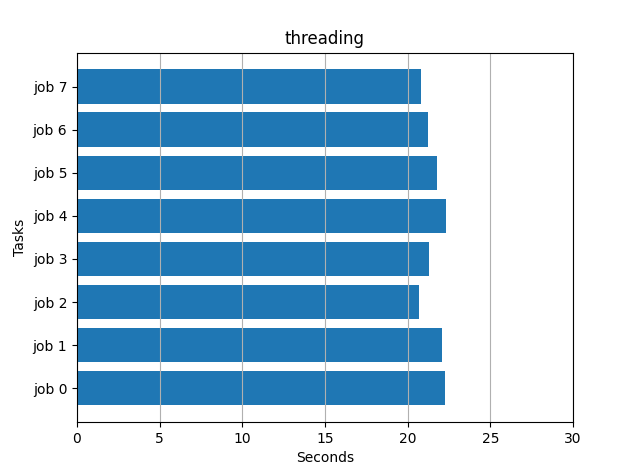
\includegraphics{zdjecia/threading_requests}
    \caption{Czasy działania threadingu przy operacji wysyłania zapytań http}
\end{figure}

\begin{figure}
    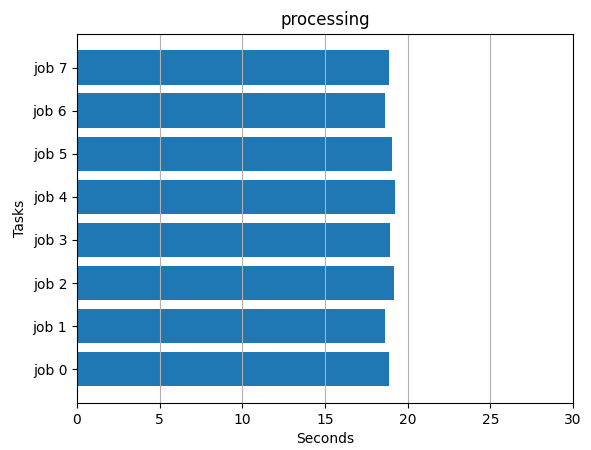
\includegraphics{zdjecia/processing_requests}
    \caption{Czasy działania multiprocessingu przy operacji wysyłania zapytań http}
\end{figure}

\begin{figure}
    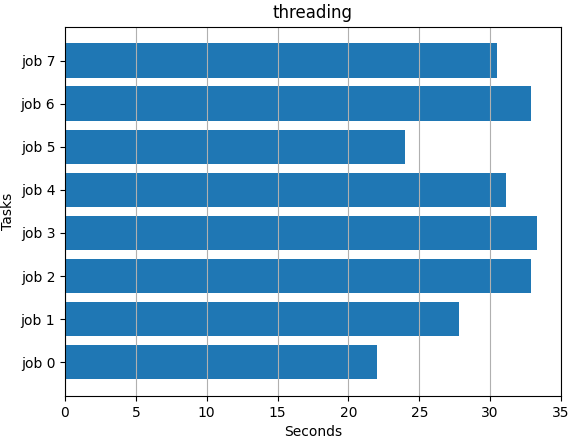
\includegraphics{zdjecia/threading_cpu}
    \caption{Czasy działania threadingu przy operacji związanej z procesorem}
\end{figure}

\begin{figure}
    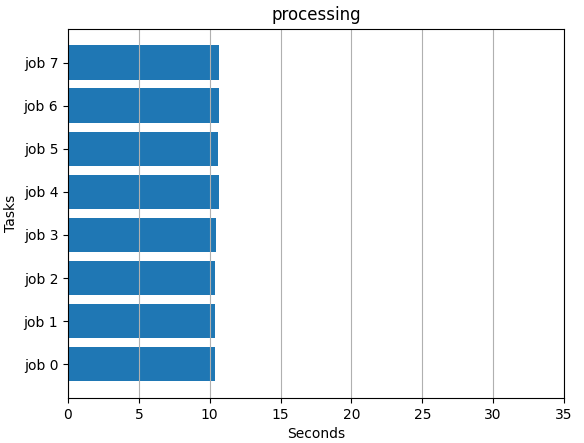
\includegraphics{zdjecia/processing_cpu}
    \caption{Czasy działania multiprocessingu przy operacji zwiżanej z procesorem}
\end{figure}

\chapter{Implementacja}

Po zapoznaniu się z ogólnym zasadami rządzacymi światem programowania współbieżnego i z samym językiem Python, przejść możemy do konkretnych implementacji mikroserwisów, które unaocznią nam jak opisane techniki mogą być używane w praktyce. Biorąc pod uwagę, że w języku Python najczęściej występującym przypadkiem wykorzystania zrównoleglenia są operacje wykonywania zapytań do zewnętrznych serwisów, zaczniemy od implementacji właśnie tego typu zastosowania.


\section{FastAPI}
Framework webowy FastAPI to projekt, który istnieje dość krótko nawet jak na realia współczesnych technologii webowych, których scena zmienia się niemal z dnia na dzień. Potrzeba na jego stworzenie powstała u jego autora nie dalej niż w roku 2018.  Tworząc komleksowe API i dowodząc kilkoma zespołami programistów Sebastian Ramirez - bo tak nazywa się twórca tego frameworka - doszedł do wniosku, że biorąc co najlepsze z wielu narzędzi, którymi się posługiwał może stworzyć technologię pozwalającą usprawnić pracę. Tak właśnie czerpiąc inspiracje z technologii takich jak Django, Django Rest Framework, Flask, Requests, Marshmallow, a nawet JavaScriptowych NestJS i Angular.

\subsection{Przykład użycia technologii}
Pracę z frameworkiem zaczynamy od instalacji samego frameworka oraz servera ASGI:
\begin{lstlisting}
pip install fastapi, uvicorn
\end{lstlisting}
Po tym podstawowym kroku możemy przejśc do konkretnej implementacji naszego mikroserwisu. Tworzymy plik o nazwie main.py i w jego treści umieszczamy:

\begin{lstlisting}
from fastapi import FastAPI

app = FastAPI()

@app.get('/')
def home():
    return {'welcome_text': 'Welcome to FastAPI showcase project'}
\end{lstlisting}

Stworzenie aplikacji ogranicza się do utworzenia instacji zaimportowanej klasy FastAPI. Następnie metody utworzonej instacji mogą być używane jako dekoratory dla konkretnych funkcji przettwarzających żądanie i zwracających konkretny response. Tak przygotowaną podstawową aplikację możemy od razu włączyć lub nawet wdrożyć. Aby włączyć aplikację możemy z terminala użyć zainstalowanego serwera ASGI poleceniem:
\begin{lstlisting}
uvicorn main:app --reload --port 8000
\end{lstlisting}
, w którym to poleceniu 'main' odpowiada nazwie pliku (modułu), w którym zainicjalizowana jest nasza aplikacja, ':app' określa nazwę zmiennej w której znajduje się instancja naszej aplikacji. Pozostałe parametry to '--reload', który w wypadku włączenia aplikacji lokalnie w czasie rozwijania będzie przeładowywał aplikacje po każdej zmianie kodu wewnątrz modułu, zaś '--port' pozwala nam określić na jakim porcie aplikacja będzie dostępna.

Przy nieco bardziej zaawansowanej strukturze projektu niezbędne będzie użycie routerów, które pozwolą nam podzielić aplikacje na kilka części. Aby użycie kilku routerów było możliwe musimy utworzyć wewnątrz struktury projektu nowy pythonowy moduł i dowolnie go nazwać. W naszej aplikacji będzie to moduł 'routers'. Wewnątrz modułu tworzymy plik o nazwie "example\_router.py" i wewnątrz pliku umieszczamy następujący kod

\begin{lstlisting}
from fastapi import APIRouter

router = APIRouter()

@router.get('/router')
async def router_example():
    return {'welcome_text': 'Welcome to FastAPI router'}
\end{lstlisting}
zaś w pliku main.py dodajemy linijki:
\begin{lstlisting}
from routers.api_requests import router as example_router
\end{lstlisting}
oraz po stworzeniu instancji FastAPI - app:
\begin{lstlisting}
app.include_router(example_router)
\end{lstlisting}
Po dodaniu tych elementów możemy otworzyć przeglądarkę internetową na adresie 'http://127.0.0.1:8000' lub 'http:127.0.0.1:8000/router', które to adresy powinny wyświetlić nam odpowiednio napisy \{'welcome\_text': 'Welcome to FastAPI showcase project'\} oraz \{'welcome\_text': 'Welcome to FastAPI router'\}.

\subsection{Operacje IO}
Pierwszym przykładem zastosowania zrównoleglania w moim projekcie będzie wykonywania zapytań na inny endpoint. 
\subsubsection{Sekwencyjnie}
Dla uproszczenia nasze api będzie wykonywało request do siebie samego, na endpoint, który po prostu zwraca napis, co nie powinno zbyt mocno dodatkowo obciążać aplikacji i wpływać zbyt mocno na finalne wyniki. Aby mieć punkt odniesienia rozpoczniemy od implementacji tego typu endpointa, który będzie wykonywał zamierzoną pracę w trybie sekwencyjnym:
\begin{lstlisting}
from fastapi import APIRouter

router = APIRouter()

@router.get('/fetch-sites-sync')
def fetch_sites_sync():
    responses = []
    for i in range(NUMBER_OF_REQUEST):
        responses.append(requests.get(URL_TO_BE_REQUESTED).content)
    return responses
\end{lstlisting}
Zmienne oznaczone wielkimi literami możemy zdefiniować dowolnie, jednak NUMBER\_OF\_REQUEST powinno być liczbą, zaś URL\_TO\_BE\_REQUESTED powinien być napisem zawierającym prawidłowy, istniejący adres internetowy.

Do wykonywania zpaytań używamy biblioteki requests. W pętli o określonej ilości przebiegów nasz kod wykonuje zapytanie i czeka na jego wynik, po czym przechodzi do kolejnego zapytania. To podejście klasyczne, które sprawdza się gdy zapytań nie jest zbyt wiele i możemy sobie pozwolić na bierne oczekiwanie.

Jeśli założymy, że jako URL\_TO\_BE\_REQUESTED podamy adres endpointa z pierwszego przykładu w tym rozdziale, a NUMBER\_OF\_REQUEST zdefinujemy jako liczbę 5, to odpwiedź z właśnie utworzonego kodu powinna być napisem \{'welcome\_text': 'Welcome to FastAPI showcase project'\} powtórzonym 5 razy.

\subsubsection{threading}
Aby skorzystać z pythonowego threadingu tworzymy następujący kod:
\begin{lstlisting}
from fastapi import APIRouter
from concurrent.futures import ThreadPoolExecutor,

router = APIRouter()

@router.get('/fetch-sites-threading')
def fetch_sites_threading():
    with ThreadPoolExecutor() as ex:
        res = ex.map(get_response_body, (URL_TO_BE_REQUESTED for _ in range(NUMBER_OF_REQUEST)))
    return res
\end{lstlisting}

W tym przykładzie używamy klasy ThreadPoolExecutor pochodzącej z modułu concurrent.futures. Moduł ten udostępnia użytkownikom języka wysokopoziomowe interejsy umożliwiające prostsze wykonywanie asynchronicznych procesów. Pod spodem używane są mechanizmy znane z modułów threading oraz processing. Stosowana w tym przykładzie klasa pozwala na korzystanie ze zbioru wątków, by wykonywać z ich pomocą zadania asynchroniczne.

W przykładach współbieżnych wykorzystujących threading oraz multiprocessing (pomijając asyncio) będziemy wykorzystywali funkcję pomocniczą o nazwie get\_response\_body zdefiniowaną następująco:
\begin{lstlisting}
import requests

def get_response_body(url):
    return requests.get(url).content
\end{lstlisting}

W przeciwieństwie do przykładu sekwencyjnego nie używamy tutaj jawnie pętli for. Zamiast tego używamy klasy ThreadPoolExecutor i do metody 'map' instacji executora powstałej w wyniku użycia klasy jako context managera przekazujemy jako pierwszy argument funkcję, która ma być wykonana asynchronicznie, zaś jako drugi argument obiekt dający się iterować. Elementy drugiego argumentu będą użyte jako argumenty funkcji, podanej jako pierwszy argument.

Przy tworzeniu instancji klasy ThreadPoolExecutor możemy podać jako pierwszy argument liczbę, która będzie reprezentowała maksymalną liczbę wątków w zbiorze używanym przez stworzony executor. Jeśli nie podamy tego argumentu domyślnie podana będzie liczba wyliczana według wzoru: 
\[ cpu * 5 \]
, gdzie przez cpu oznaczamy liczbę procesorów (lub rdzeni procesora) wykrywalnych w systemie.

Wynik zapytania na ten endpoint z analogicznymi jak w pierwszym przykładzie wartościami zmiennych NUMBER\_OF\_REQUEST oraz URL\_TO\_BE\_REQUESTED powinna być identyczna jak w przykładzie sekwencyjnym, zmianie powinien ulec jedynie czas wykonania, który powinien być krótszy i wynosić czas wykonania nadłuższego zapytania. Założenie to będziemy sprawdzać w kolejnym rozdziale, podobnie jak inne poczynione w tym rozdziale przewidywania dotyczące wyników i czasów wykonań kodu tworzonych endpointów.

\subsubsection{multiprocessing}
W celu posłużenia się mechanizmem tworzenia oddzielnych procesów w FastAPI posłużymy się następującym kodem:
\begin{lstlisting}
from fastapi import APIRouter
from concurrent.futures import ThreadPoolExecutor,

router = APIRouter()

@router.get('/fetch-sites-threading')
def fetch_sites_threading():
    with ProcessPoolExecutor() as ex:
        res = ex.map(get_response_body, (URL_TO_BE_REQUESTED for _ in range(NUMBER_OF_REQUEST)))
    return res
\end{lstlisting}

Jedyna jawna różnica względem endpointa korzystającego z threadingu to użyta klasa executora - zmiana z ThreadPoolExecutora na ProcessPoolExecutora sprawia, że zamiast używania wątków kod będzie korzystał z zupełnie oddzielnych procesów. Mówiąc inaczej, niejawnie zamiast modułu threading będzie używany moduł multiprocessing. Tutaj opcjonalny argument przy inicjalizacji klasy to liczba reprezentująca maksymalną liczbę robotników wykonujących pracę równolegle. W tym przypadku domyślna wartość jeśli programista nie poda swojej to dokładnie ilość procesorów lub rdzeni procesora.

Ponownie wynik zapytania z analogicznymi wartościami zmiennych powinien być identyczny, zaś czas wykonania podobny do przypadku z użyciem wątków, prawdopodobnie z naddatkiem związanym z koniecznością włączenia oddzielnego procesu dla każdego wykonania.
\chapter{Eksperymenty}

W tym rozdziale przedstawię wyniki kilku prób użycia aplikacji opisanych w poprzednim rozdziale. Próby będę przeprowadzał z użyciem narzędzia ,,siege''\footnote{\url{https://www.joedog.org/siege-home/}, \url{https://github.com/JoeDog/siege}}. Jest to otwarto-źródłowa technologia do wykonywania testów obciążenia aplikacji webowych. W wynikach działania programu będziemy mogli odczytać całkowitą liczbę wykonanych zapytań, liczbę przesłanych bajtów, czas odpowiedzi, współbieżność odpowiedzi oraz kod odpowiedzi. Parametrami dla nas najważniejszymi będzie czas odpowiedzi, całkowity czas wykonania konkretnej liczby zapytań i oczywiście zależy nam by kod odpowiedzi był zawsze prawidłowy. Co więcej narzędzie to umożliwia wysyłanie kilku zapytań współbieżnie, imitując wielu współbieżnych użytkowników naszej strony.

\section{uruchomienie aplikacji}
Usługę zaimplementowaną w FastAPI wystawiamy poleceniem:
\begin{lstlisting}
gunicorn main:app -w 4 -k uvicorn.workers.UvicornWorker -b localhost:8080
\end{lstlisting}
znajdując się oczywiście w katalogu fastapi\_examples. Użyjemy czterech workerów pochodzących z ,,uvicorna'', gdyż umożliwiają one pracę z widokami asynchronicznymi. Usługę ,,przypinamy'' do portu 8080 naszego serwera, aby odróżnić ją od tej wystawionej w Django na porcie 8000.

Aby uzyskać jak najbardziej zbliżone warunki działania komenda do włączenia serwisu wykonanego w Django będzie bardzo zbliżona:
\begin{lstlisting}
gunicorn django_examples.asgi:application -w 4 -k uvicorn.workers.UvicornWorker
\end{lstlisting}
Oczywiście komenda również wykonywana z wnętrza katalogu, w którym rezydują pliki naszej aplikacji.

\section{Widoki wysyłające zapytania}
\subsection{Sekwencyjnie}
Zaczniemy od pojedynczego zapytania jednego użytkownika. W tym celu wykonujemy komendę:
\begin{lstlisting}
siege http://127.0.0.1:8080/fetch-sites-sync -c1 -r1
\end{lstlisting}
gdzie parametr -c to liczba współbieżnych użytkowników, zaś -r to liczba kolejnych requestów jakie ma wykonać każdy z nich. Wynik naszej komendy jest następujacy:
\begin{figure}[H]
    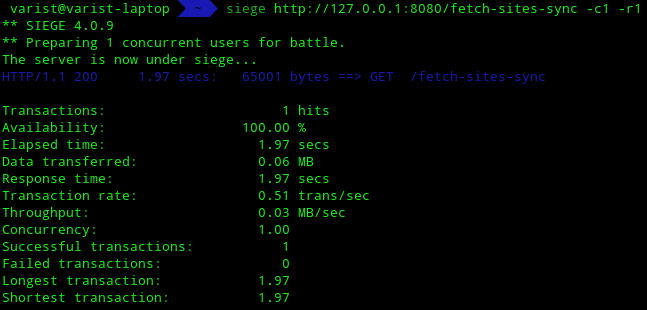
\includegraphics[height=50mm]{zdjecia/1_req_sync_fast}
    \centering
\end{figure}
Zostało wykonane dokładnie jedno zapytanie na endpoint ,,/fetch-sites-sync''. Czas jaki zajęło wykonanie tego zapytania i otrzymania odpowiedzi to 1.89 sekundy, podobnie jak całego procesu wysyłania zapytań i odbierania odpowiedzi.

Aby zobaczyć jak ta sama operacja wykona się w Django w poprzednim poleceniu zmieniamy jedynie port na odpowiadający temu, na którym działa serwis wykonany w Django:
\begin{figure}[H]
    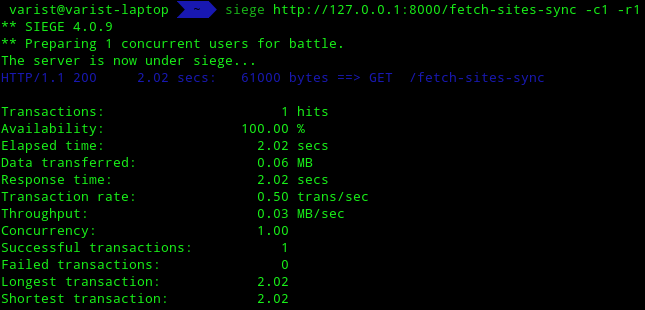
\includegraphics[height=50mm]{zdjecia/1_req_sync_django}
    \centering
\end{figure}

Teraz, aby osiągnąć nieco bardziej reprezentatwyne wyniki zasymulujemy wykonanie tego zapytania przez 10 użytkowników współbieżnie, z których każdy będzie wykonywał po 5 zapytań.
\begin{figure}[H]
    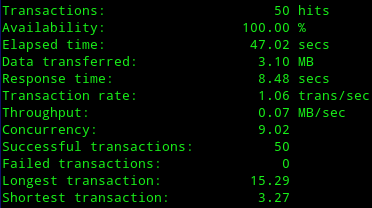
\includegraphics[height=50mm]{zdjecia/10_req_sync_fast}
    \centering
    \caption{FastAPI, 10 użytkowników, 5 zapytań}
\end{figure}

\begin{figure}[H]
    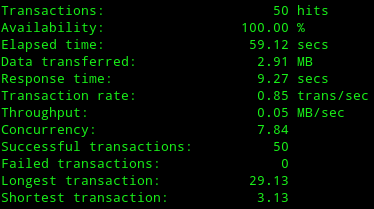
\includegraphics[height=50mm]{zdjecia/10_req_sync_django}
    \centering
    \caption{Django, 10 użytkowników, 5 zapytań}
\end{figure}

Wniosek: Rozbudowanie Django sprawia, że już w wypadku prostego sekwencyjnego wykonania zapytań proces trwa dłużej, gdyż każde zapytanie musi przejść nieco dłuższą drogę. Prawdopodobnym czynnikiem zmniejszającym wydajność Django może być też praca wykonywanay przez klasę JsonResponse, która jest odpowiedzialna za przełożenie otrzymanych odpowiedzi na notację JSON\footnote{JavaScript Object Notation}, jednak spore znaczenie na pewno mają tez wbudowane middleware'y.

\subsection{threading}
Teraz zaczniemy od testu endpointów używających modułu threading od razu używając opcji dziesięciu użytkowników i pięciu zapytań. Zaczynając od FastAPI:
\begin{figure}[H]
    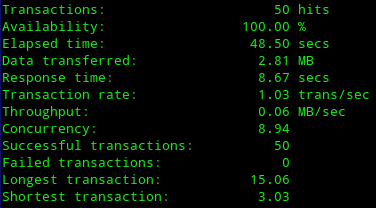
\includegraphics[height=50mm]{zdjecia/10_req_thread_fast}
    \centering
    \caption{FastAPI, threading, 10 użytkowników, 5 zapytań}
\end{figure}

\begin{figure}[H]
    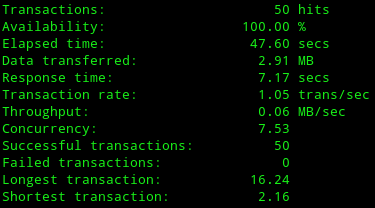
\includegraphics[height=50mm]{zdjecia/10_req_thread_django}
    \centering
    \caption{Django, threading, 10 użytkowników, 5 zapytań}
\end{figure}
Zaobserwować możemy, że przewaga FastAPI, którą widzieliśmy w przykładzie sekwencyjnym tutaj się ulotniła. Związane jest to z mechanizem FastAPI, który decyduje o tym czy widok zdefiniowany jest jako ,,async def'' czy też zwykły ,,def'' przez co w przypadku threadingu oba frameworki wypadają podobnie. Korzystniej wypadałoby użycie widoku zdefiniowanego jako ,,async def'' w FastAPI, jednak w przypadku korzystania z threadingu wewnątrz tak zdefiniowanych widoków rodziłoby się niebezpieczeństwo związane z wyciekami pamięci i zatrzymaniem niektórych wątków, a co za tym idzie utratą części przesłanych danych. Byłoby to rozwiązanie możliwe do implementacji, jeśli możemy pozwolić klientowi naszego api na powtórzenie zapytania w wypadku otrzymania błędu. Należałoby wtedy ocenić korzyści czasowe płynące z zastosowania takiego rozwiązania wobec strat związanych z ponawianiem zapytań.

\subsection{multiprocessing}
\begin{figure}[H]
    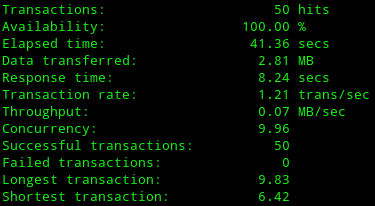
\includegraphics[height=50mm]{zdjecia/10_req_process_fast}
    \centering
    \caption{FastAPI, multiprocessing, 10 użytkowników, 5 zapytań}
\end{figure}

\begin{figure}[H]
    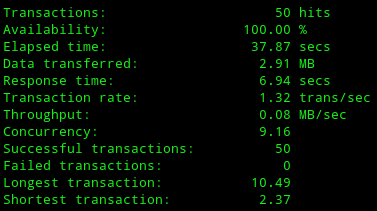
\includegraphics[height=50mm]{zdjecia/10_req_process_django}
    \centering
    \caption{Django, multiprocessing, 10 użytkowników, 5 zapytań}
\end{figure}

Tutaj ponownie przewaga uzyskana przez FastAPI przy klasycznym sekwencyjnym podejściu została zniwelowana. Multiprocessing stanowczo w obu frameworkach działa tak samo dobrze, nawet z lekkim wskazaniem w stronę Django, które przypomnijmy miało być w tym starciu technologią bardziej rozbudowaną, ale jednak wolniejszą. Warto podkreślić, że tak dobry wynik tego rozwiązania nie byłby możliwy bez zastosowania go na architekturze opartej o kilkurdzeniowy procesor.

\subsection{asyncio}
\begin{figure}[H]
    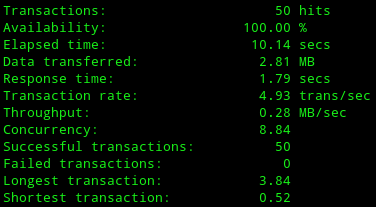
\includegraphics[height=50mm]{zdjecia/10_req_asyncio_fast}
    \centering
    \caption{FastAPI, asyncio, 10 użytkowników, 5 zapytań}
\end{figure}

\begin{figure}[H]
    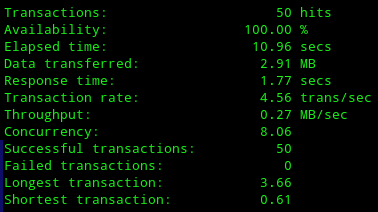
\includegraphics[height=50mm]{zdjecia/10_req_asyncio_django}
    \centering
    \caption{Django, asyncio, 10 użytkowników, 5 zapytań}
\end{figure}
Zgodnie z przewidywaniem technologia asyncio w przypadku tego typu operacji bije konkurencję na głowę. Wzrost wydajności o niemal 40 sekund względem rozwiązania z zastosowaniem threadingu i niemal 30 sekund względem multiprocessingu. Co ciekawe w obu frameworkach czas wykonania jest bardzo zbliżony i różni się o niecałą sekundę. W perspektywie 10 sekund, które zajął cały proces jest to różnica niecałych 10\% na korzyść młodszego frameworka.

\section{Obliczenia}
\subsection{Sekwencyjnie}
Ponownie rozpoczniemy od obejrzenia wyniku wysłania pojedynczego zapytania na endpoint wykonujący przewidywane obliczenia w trybie całkowicie sekwencyjnym.
\begin{figure}[H]
    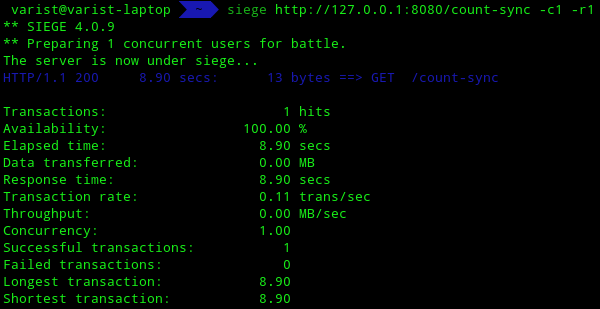
\includegraphics[height=50mm]{zdjecia/1_math_sync_fast}
    \centering
    \caption{FastaAPI, sekwencyjnie, 1 użytkownik, jedno zapytanie}
\end{figure}

\begin{figure}[H]
    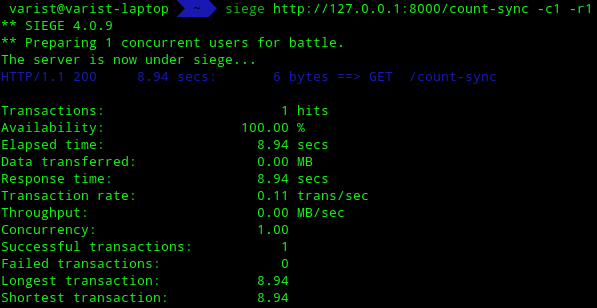
\includegraphics[height=50mm]{zdjecia/1_math_sync_django}
    \centering
    \caption{Django, sekwencyjnie, 1 użytkownik, jedno zapytanie}
\end{figure}
Możemy zaobserwować, że w wypadku obliczeń matematycznych frameworki zachowują się praktycznie identycznie, wynik czasowy różni się o 4 setne sekundy, co przy całkowitym wyniku oscylującym w granicach 8-9 sekund jest wartością pomijalną. Sprawdźmy jednak czy w sytuacji wysłania wielu zapytań sytuacja nie ulegnie zmianie.
\begin{figure}[H]
    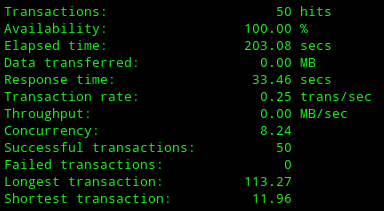
\includegraphics[height=50mm]{zdjecia/10_math_sync_fast}
    \centering
    \caption{FastAPI, sekwencyjnie, 10 użytkowników, 5 zapytań}
\end{figure}

\begin{figure}[H]
    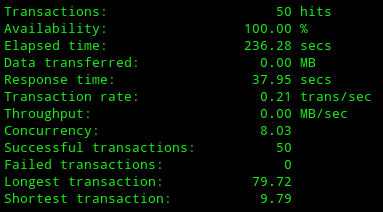
\includegraphics[height=50mm]{zdjecia/10_math_sync_django}
    \centering
    \caption{Django, sekwencyjnie, 10 użytkowników, 5 zapytań}
\end{figure}
Tutaj kwestia wygląda nieco ciekawiej niż w wypadku wysyłania zapytań. Całościowy czas wykonania wszystkich zapytań przez wszystkich użytkowników okazał się być lepszy w wypadku FastAPI - 203 sekundy względem 236 sekund w Django. Co ciekawe jednak zarówno najdłuższy jak i najkrótszy cykl zapytanie-odpowiedź w wypadku FastAPI są znacząco dłuższe niż analogiczne wskaźniki w Django, pomimo że oczywiście średni czas takiego cyklu jest krótszy w FastAPI. Świadczy to o mniej stabilnej pracy wynikowej frameworka i sprawia, że pomimo satysfakcjonującej prędkości jest on w wypadku rozwiązań sekwencyjnych mniej niezawodny.

\subsection{threading}
Zobaczmy jak widoki wykonujące zasobożerne obliczenia będą się zachowywały, gdy do próby ich zrównoleglenia użyjemy threadingu.
\begin{figure}[H]
    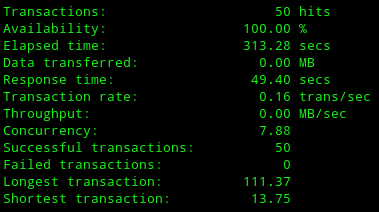
\includegraphics[height=50mm]{zdjecia/10_math_thread_fast}
    \centering
    \caption{FastAPI, threading, 10 użytkowników, 5 zapytań}
\end{figure}

\begin{figure}[H]
    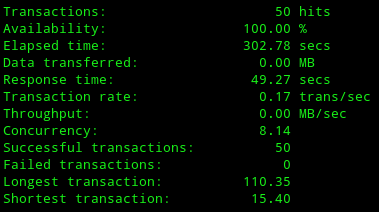
\includegraphics[height=50mm]{zdjecia/10_math_thread_django}
    \centering
    \caption{Django, threading, 10 użytkowników, 5 zapytań}
\end{figure}
W tym przypadku jak widać sytuacja jest dużo bardziej zbliżona. Czasowo ze wszystkimi zapytaniami lepiej poradziło sobie Django, jednocześnie nieco lepiej wypadając również w kwestii najrótszego oraz nadłuższego zapytania. Choć różnica tutaj nie jest tak duża, to jednak zaskakującym jest, że ponownie znajduje się aspekt, w którym starszy framework radzi sobie lepiej.

\subsection{multiprocessing}
Warto nadmienić, że według oczekiwań multiprocessing powinien być rozwiązaniem, które w przypadku wykonywania obliczeń matematycznych powinien w środowisku wielordzeniowym poradzić sobie najlepiej. Sprawdźmy czy to przewidywanie jest słuszne.
\begin{figure}[H]
    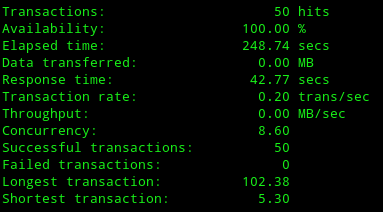
\includegraphics[height=50mm]{zdjecia/10_math_process_fast}
    \centering
    \caption{FastAPI, multiprocessing, 10 użytkowników, 5 zapytań}
\end{figure}

\begin{figure}[H]
    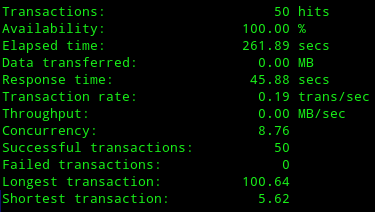
\includegraphics[height=50mm]{zdjecia/10_math_process_django}
    \centering
    \caption{Django, multiprocessing, 10 użytkowników, 5 zapytań}
\end{figure}
Multiprocessing poradził sobie widocznie lepiej niż threading. Wzrost prędkości jest między tymi dwoma rozwiązaniami wyraźny, jednak ciekawą obserwacją jest to, że multiprocessing wypadł słabiej niż rozwiązanie sekwencyjne korzystające z jednego wątku. Wyjaśnienie takiego stanu rzeczy jest dość proste. Stosując rozwiązanie jakim jest serwer gunicorn włączane są cztery procesy - parametr -w wskazuje nam jaka dokładnie liczba workerów powinna pracować cały czas. Oznacza to że w zasadzie już z założenia gunicorna nasza aplikacja jest aplikacją wieloprocesową, a dodanie dodatkowych procesów wewnątrz endpointa powoduje jedynie dodatkowy narzut jaki system musi wykonać by nimi zarządzać. Sytuacja oczywiście byłaby inna, gdybyśmy dysponowali maszyną o bardzo wielu rdzeniach, lecz przy naszym zastosowaniu - warto pomyśleć o innym rozwiązaniu.

\subsection{asyncio}
\begin{figure}[H]
    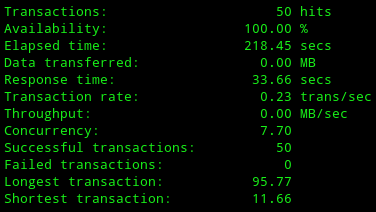
\includegraphics[height=50mm]{zdjecia/10_math_asyncio_fast}
    \centering
    \caption{FastAPI, asyncio, 10 użytkowników, 5 zapytań}
\end{figure}

\begin{figure}[H]
    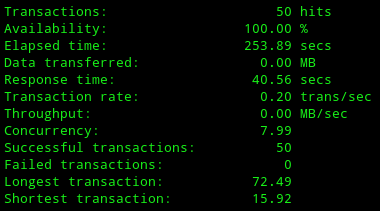
\includegraphics[height=50mm]{zdjecia/10_math_asyncio_django}
    \centering
    \caption{Django, asyncio, 10 użytkowników, 5 zapytań}
\end{figure}
Już szybki rzut oka na powyższe wyniki pozwala nam odczytać, że niekwestionowanym zwycięzcą spośród naszych mechanizmów zrównoleglania jest asyncio. Bez wątpienia jest to technologia, która w naszym przypadku użycia spisała się najlepiej, wciąż jednak nieco gorzej niż rozwiązanie sekwencyjne. Ponadto dużo lepiej w użyciu asyncio wypadło FastAPI - różnica aż o około 20\% sprawia, że jeśli chcieć używać asynchroniczności w kontekście aplikacji webowych - FastAPI powinno być naszym pierwszym wyborem.

\section{Wnioski}

Podsumowując przeprowadzone we wcześniej części tego rozdziału testy stworzyłem następującą tabelę prezentującą wyniki czasowe widoków wysyłających zapytania. Widać tutaj lekką przewagę nieco bardziej doświadczonego frameworka jakim jest Django, jednak przewaga ta jest widoczna jedynie w technologiach uruchamianych w kontekście sekwencyjnym, a także tam gdzie używane są mechanizmy threading oraz multiprocessing. Już natomiast w wypadku użycia asyncio przewaga zmienia się na korzyść nowocześniejszego frameworka. 

\begin{table}[ht]
\caption{Wyniki czasowe wysyłania zapytań}
\centering
\begin{tabular}{c c c c}
\hline\hline
Mechanizm & FastAPI & Django \\ [0.5ex]

\hline
Sekwencyjnie & 47.02s & 59.12s \\
threading & 48.50s & 47.60s \\
multiprocessing & 41.36 & 37.87s \\
asyncio & 10.14 & 10.96s \\[1ex]
\hline
\end{tabular}
\end{table}

Druga tabela w tej części to już wyniki podsumowujące pracę frameworków w kontekście wykonywania pracy obliczeniowej związanej z Centralną Jednostką Obliczeniową naszego serwera.
\begin{table}[ht]
\caption{Wyniki czasowe obliczeń}
\centering
\begin{tabular}{c c c c}
\hline\hline
Mechanizm & FastAPI & Django \\ [0.5ex]

\hline
Sekwencyjnie & 203.08s & 236.28s \\
threading & 313.28s & 302.78s \\
multiprocessing & 248.74 & 261.89s \\
asyncio & 218.45s & 253.89s \\[1ex]
\hline
\end{tabular}
\end{table}

Tutaj jak już wspominałem wyniki są dość zaskakujące. Sporą część pracy, którą w normalnej sytuacji wykonywałyby mechanizmy zrównoleglające - tutaj wykonywana jest przez workery, którymi posługuje się nasza aplikacja.

W tym przypadku również różnica między frameworkami nie jest tak oczywista - pomimo użycia dokładnie tych samych parametrów wyniki czasowe są zróżnicowane. W rozwiązaniu sekwencyjnym lepiej z rozporządzaniem mocą obliczeniową poradziło sobie FastAPI, przy użyciu threadingu niewielką przewagę uzyskało Django, zaś odwrotna sytuacja zaistniała w przypadku multiprocessingu. Niekwestionowanym słusznym rozwiązaniem w przypadku użycia asyncio jest framework FastAPI - tutaj sytuacja jest bardzo zbliżona do opcji z części wysyłającej zapytania i nie ma wątpliwości, że jeśli przy projektowaniu architektury naszego programu wiemy, że będziemy korzystać z asynchronicznych funkcjonalności Pythona to nasz wybór powinien paść na FastAPI, w przeciwnym wypadku zaś - skłonić się powinniśmy ku Django.


\clearpage
\bibliography{main}
\bibliographystyle{ieeetr}

\clearpage


\end{document}
